\documentclass[10pt,hyperref={CJKbookmarks=true},xcolor=dvipsnames,aspectratio=169]{beamer}
\usetheme[navigation]{UMONS}
\usepackage[utf8]{inputenc}
\usepackage{verbatim}
\usepackage{ctex}

\title[国际经济学]{国际经济学}
\subtitle{欧洲货币体系与欧元}
\author{鲁晓东}
\institute[]{%
	岭南学院\hspace{2em}中山大学
	\\[4ex]
	
\includegraphics[height=8ex]{fig/lingnanlogo}\hspace{2em}%
	
\includegraphics[height=8.5ex]{fig/sysu}
}
%------------section前展示一页----------
\AtBeginSection[] {     
	\begin{frame}        
	\tableofcontents[currentsection,hideallsubsections]    
\end{frame} 
}

%-------------subsection也展示一下----------
\AtBeginSubsection[]{

\frame<beamer>{ 
	
	\frametitle{Outline}   
	
	\tableofcontents[currentsection,currentsubsection] 
	
}

}
%---------------------------

%-----------一段一闪现-------
%\beamerdefaultoverlayspecification{<+->}
%这个功能基本不用

\begin{document}
\maketitle


\begin{frame}
\frametitle{提纲}
\tableofcontents
\end{frame}				%生成提纲页

%-----------正文开始----------------------



\section{Motivation}
\begin{frame}{From Academics to Reality}
\begin{itemize}
	\item 1961年,经济学家蒙代尔写了一篇论述货币区的论文---A Theory of Optimum Currency Areas,文章提出各国要用一种单一货币或者共同货币来替代某国货币
	\item 当时,几乎每个国家都是一个独立的货币区,因此孟德尔也怀疑他研究是否有实际意义,
	\item 什么是货币区的合适范围,最初这可能纯粹是个学术问题,因为它几乎没有进入各国政治可行性的考虑范围内,即放弃母国货币而采用另外一种安排
	\item 差不多40年之后,就在1999年,11个欧洲国家作出选择,建立这样一个货币区,现在称之为欧元区(Eruozone)
	\item 几个月以后,蒙代尔被授予诺贝尔经济学奖
	\item 此后欧元区,一次次的扩大,现在,有19个成员国,有3亿人在使用这种货币
	\item 2008年金融危机之后,冰岛、希腊、爱尔兰、葡萄牙、西班牙等国相继陷入国债危急中。2009年10月20日浮出水面的希腊债务危机为欧元危机正式拉开了序幕。
	\item 2018年,意大利出现反欧元的政治力量
	
\end{itemize}
\end{frame}
\begin{frame}{Quotation on Euro}
	\begin{block}{让$\bullet$莫内(欧洲之父)}
		除了结成联盟以外,欧洲人没有未来,
	\end{block}
	\begin{block}{《马斯特里赫特条约》(欧盟条约),1992年,第一编,第A条,}
	在创建一个欧洲各国人民之间空前紧密的联盟的进程中,本条约标志着一个新的阶段,期间的所有决策都尽可能贴近民意
\end{block}
	\begin{block}{米尔顿$\bullet$弗里德曼,诺贝尔经济学奖得主,1997年,}
	政治统一可以为货币统一铺平道路,在不利的条件下强制实施的货币统一,必定会成为达到政治统一的障碍
\end{block}


\end{frame}

\begin{frame}{欧元危机:共同货币阴影下的欧洲}
\begin{columns}[onlytextwidth]
	\begin{column}{0.6\textwidth}
		\begin{itemize}
			\item 尽管被它的设计者誉为一个能够令欧洲团结并繁荣的杠杆工具,但欧元实行的效果却大相径庭
			\item 在不同的国家中使用共同货币,致使欧元从诞生之日起就先天缺陷
			\item 经济一体化的速度超过了政治一体化的速度,直接导致了欧洲经济停滞,前景黯淡
			\item 那么,接下来的问题就是:欧元还有挽救的机会吗?
			\begin{itemize}
				\item 对欧元区结构以及对欧元区成员国施加的政策进行彻底改革
				\item 对单一货币的欧元试验进行妥善终止
				\item 或者构建一个大胆的崭新体系,即“灵活欧元”
			\end{itemize}
		\end{itemize}
	\end{column}
	\begin{column}{0.4\textwidth}
		\centering
		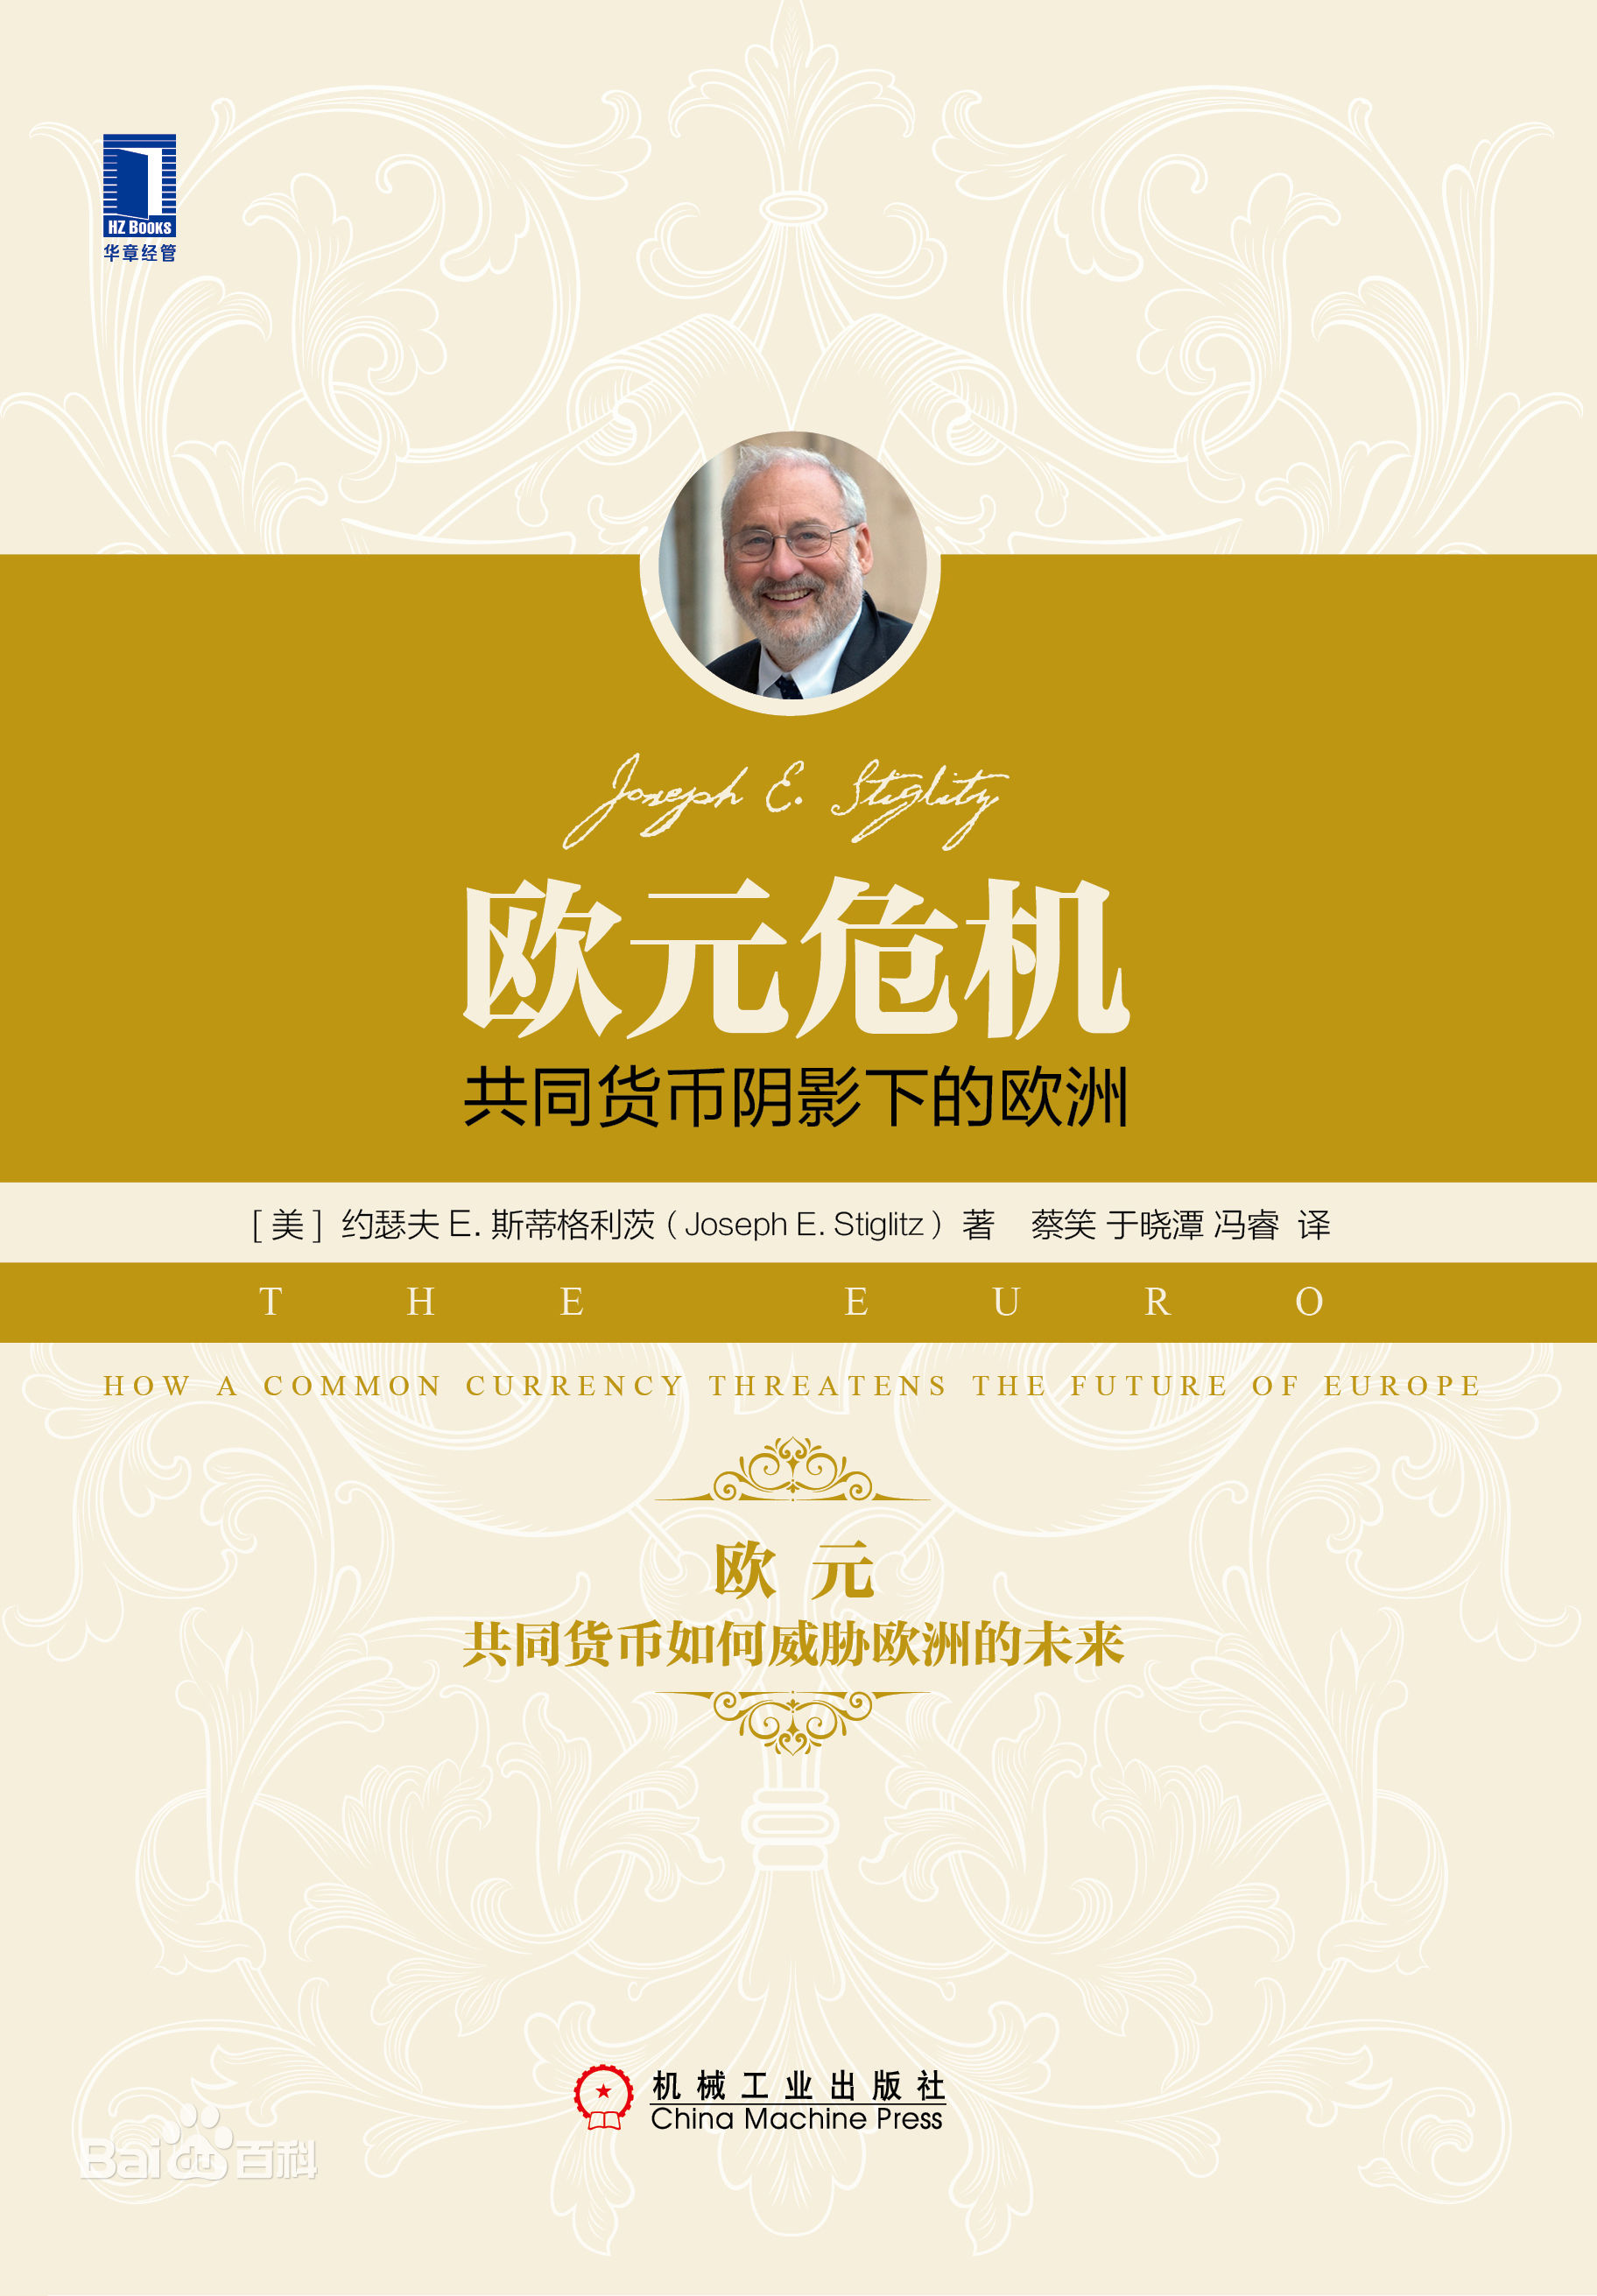
\includegraphics[scale=0.3]{fig/euro/stiglitz}
	\end{column}
\end{columns}
\end{frame}	

\begin{frame}{Who are in EU zone?}
\begin{columns}[onlytextwidth]
	\begin{column}{0.4\textwidth}
		\begin{itemize}
			\item EU-Eurozone (19): Austria, Belgium, Cyprus,
			Estonia, Finland, France, Germany, Greece,
			Ireland, Italy, Luxembourg, Malta, Netherlands,
			Portugal, Slovakia, Slovenia, Spain, Lithuania2014, Latvia2015.
			\item EU-ERM (1): Denmark.
			\item EU-Other (7): Bulgaria, Czech Republic,
			Hungary, Poland, Romania, Sweden,Croatia
			\item Candidates (4): United
			Kingdom, Iceland, Macedonia,
			Turkey.

		\end{itemize}
	\end{column}
	\begin{column}{0.6\textwidth}
		\centering
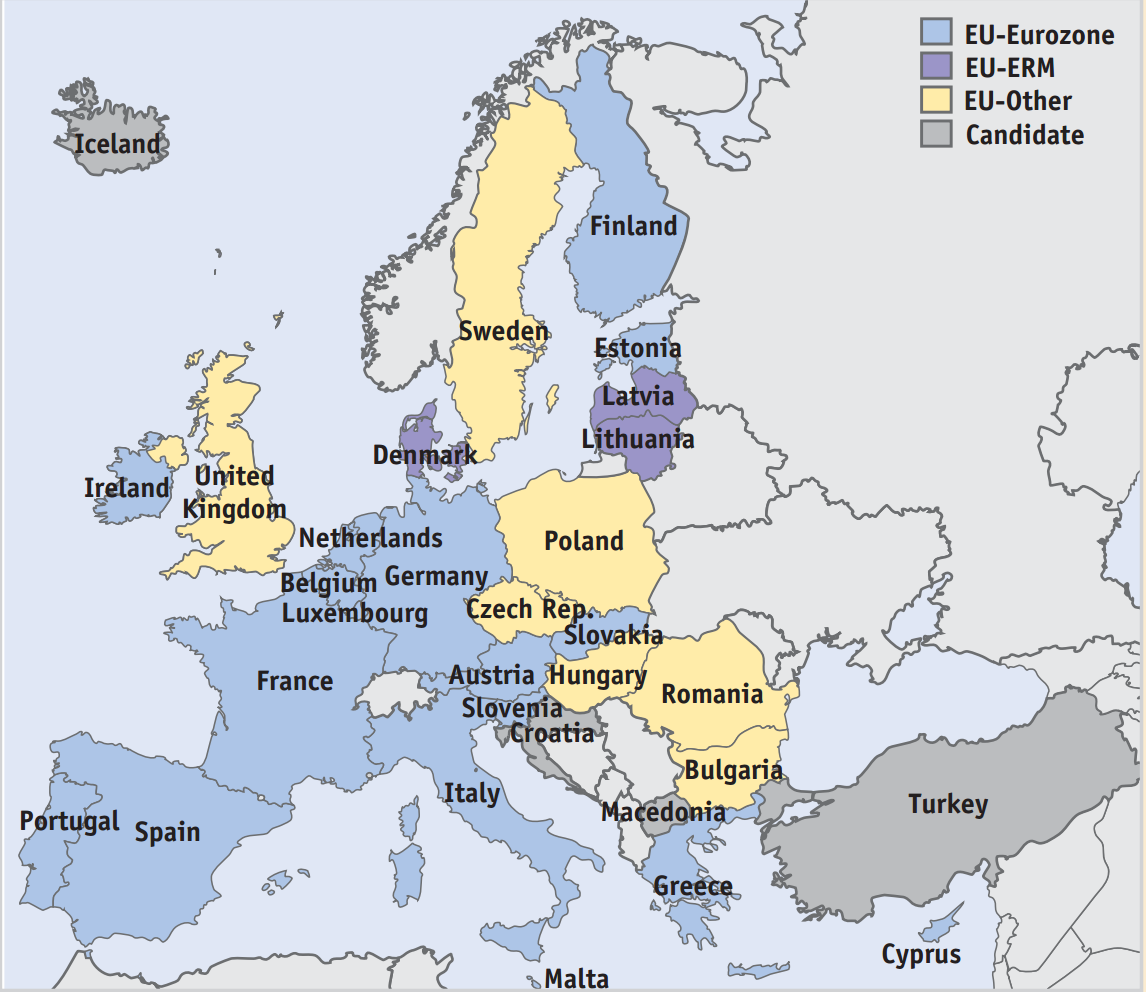
\includegraphics[scale=0.33]{fig/euro/euzone}
	\end{column}
\end{columns}

\end{frame}


\section{From Snake to the EMS}
\begin{frame}{The Snake of in the Tunnel}
	\begin{itemize}
		\item 1972-1979, Te Snake system in the Tunnel--- mini-Bretton Woods
		\item 1972-1976 the ‘worm inside the Snake’!
		\item After 1973, the plain ‘Snake’.
		\item The Snake system had a chequered history
	\end{itemize}
\end{frame}

\begin{frame}{Central parity realignments in the Snake}
		\centering
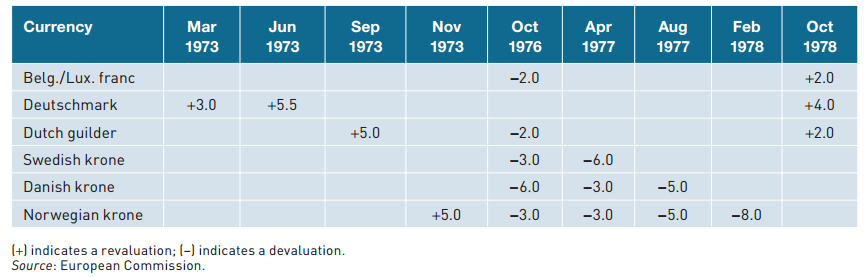
\includegraphics[scale=0.8]{fig/euro/snake}
\end{frame}

\begin{frame}{the Background of EMS}
	\begin{itemize}
		\item On 17 June 1978, at a conference held in Bremen, six of the community countries
		committed themselves to the setting-up of the EMS to replace the Snake.
		\item Te EMS commenced operation on 13 March 1979 and, despite much initial scepticism about its survival chances, operated with mixed success for two decades. 
		\item The		EMS consisted of three main features:
		\begin{enumerate}
			\item the Exchange Rate Mechanism (ERM); 
			\item the European Currency Unit (ECU)
			\item  financing facilities. A proposed European				
			\end{enumerate} 
	\end{itemize}
\end{frame}

\begin{frame}{The Features of  ERM欧洲货币体系}
\begin{itemize}
	\item A grid of bilateral exchange rate bands between each of the member currencies
	2.25--6--15
	\item An individual band of fluctuation (threshold) for each currency against the ECU
	\item  which authority was responsible for intervention when a bilateral margin was	reached?
\end{itemize}
		\centering
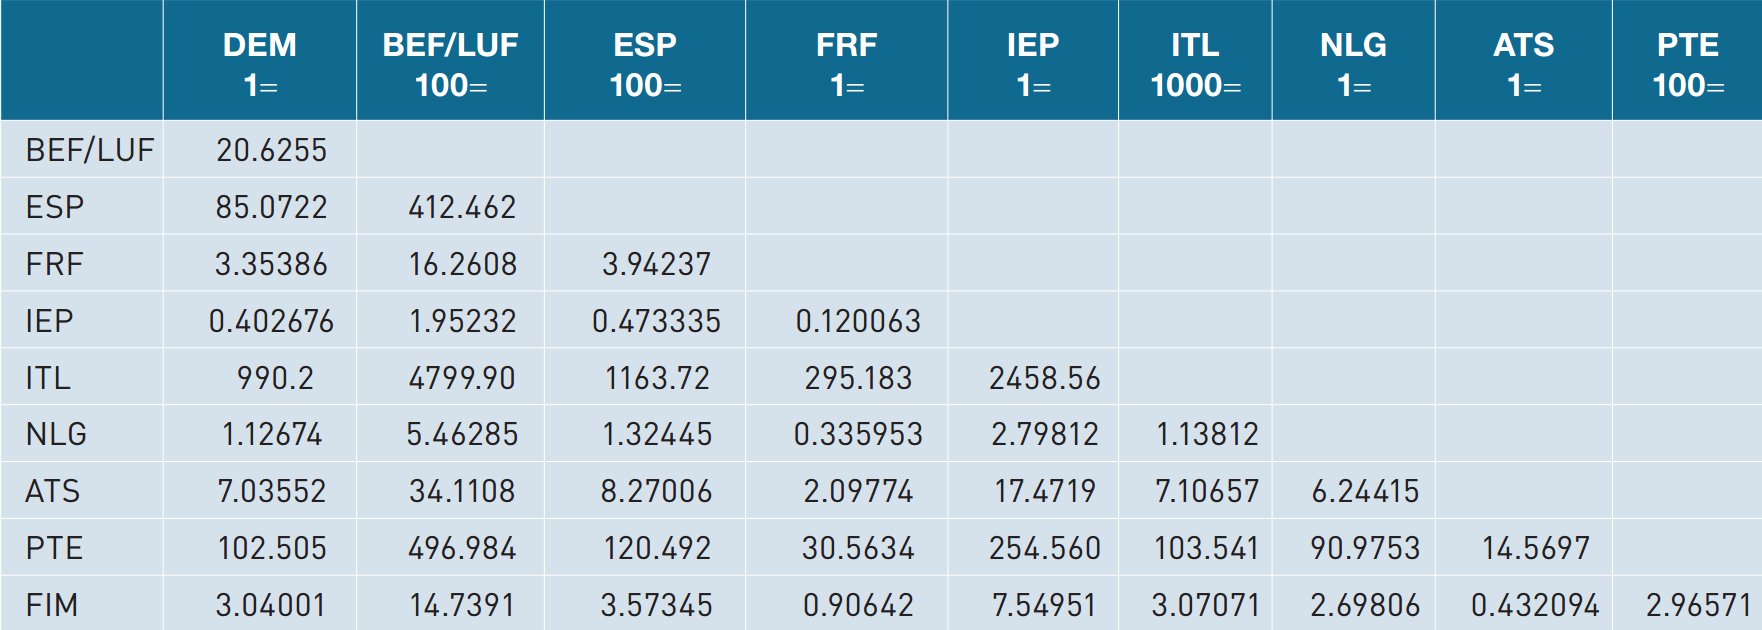
\includegraphics[scale=0.35]{fig/euro/grid}
\end{frame}

\begin{frame}{The ECU and its Role as an indicators of Divergence}
\begin{itemize}
	\item 	Te ECU埃居 was an artificial currency based upon a calculation of a weighted basket
	of 12 European currencies.
	\item The ECU was nothing more than a calculation of how a currency was doing against
	a basket of other European currencies. 
\end{itemize}
		\centering
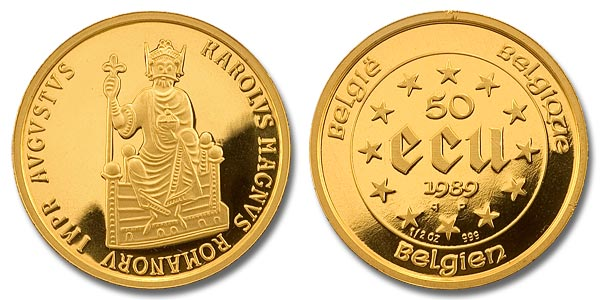
\includegraphics[scale=0.3]{fig/euro/ecu}
\end{frame}

\begin{frame}{FINANCING FACILITIES }
	\begin{itemize}
		\item  each member of the EMS deposited 20\%
		of its gold dollar reserves with the EMCF in exchange for the equivalent value in
		ECUs
		\item Adiminstrative Organization Evolution\\
		1973欧洲货币合作基金(European
		Monetary Cooperation Fund (EMCF)$\Rightarrow$1994欧洲货币管理局(European
		Monetary Institute)$\Rightarrow$1998欧洲中央银行(European System of Central Banks
		(ESCB) )
		\item credit
		facilities
		\begin{itemize}
			\item Very short-term financing ---45days
			\item Short-term monetary support---3 months
			\item Medium-term financial assistance---2-5 years
		\end{itemize}
\end{itemize}
\end{frame}

\begin{frame}{Asscessment of the EMS}
	\begin{enumerate}
		\item as a zone		of currency stability
		\begin{itemize}
			\item some critics of the system viewed it as a ‘mere			crawling peg’
			\item Despite these periodic crises, authors such as Artis and Taylor (1988, 1994)
			have shown that both nominal exchange rates and real effective exchange rates
			had become less volatile for EMS currencies (kroner, Belgian franc, lira, guilder and
			Deutschmark) than for non-EMS currencies (the pound, dollar and yen) since 1979
			compared with the first six years of floating. 
			\item countries derived both greater domestic and external financial
			stability from membership of the ERM
			
		\end{itemize}
		\item   as an anti-inflation zone
		\begin{itemize}
			\item Germany has good reputation in fighting inflation, Why?历史的惨痛教训
			\item two ways that
			the fight against inflation was assisted by full EMS membership: 
			\begin{enumerate}
				\item by giving the
				authorities an incentive to bring inflation under control
				\item by affecting private
				agents’ wage and price behaviour.
			\end{enumerate}
		\item no proof of the EMS anti-inflation
		hypothesis
		\end{itemize}
	\end{enumerate}
\end{frame}
\begin{frame}{Inflation in ERM and non-ERM countries}
		\centering
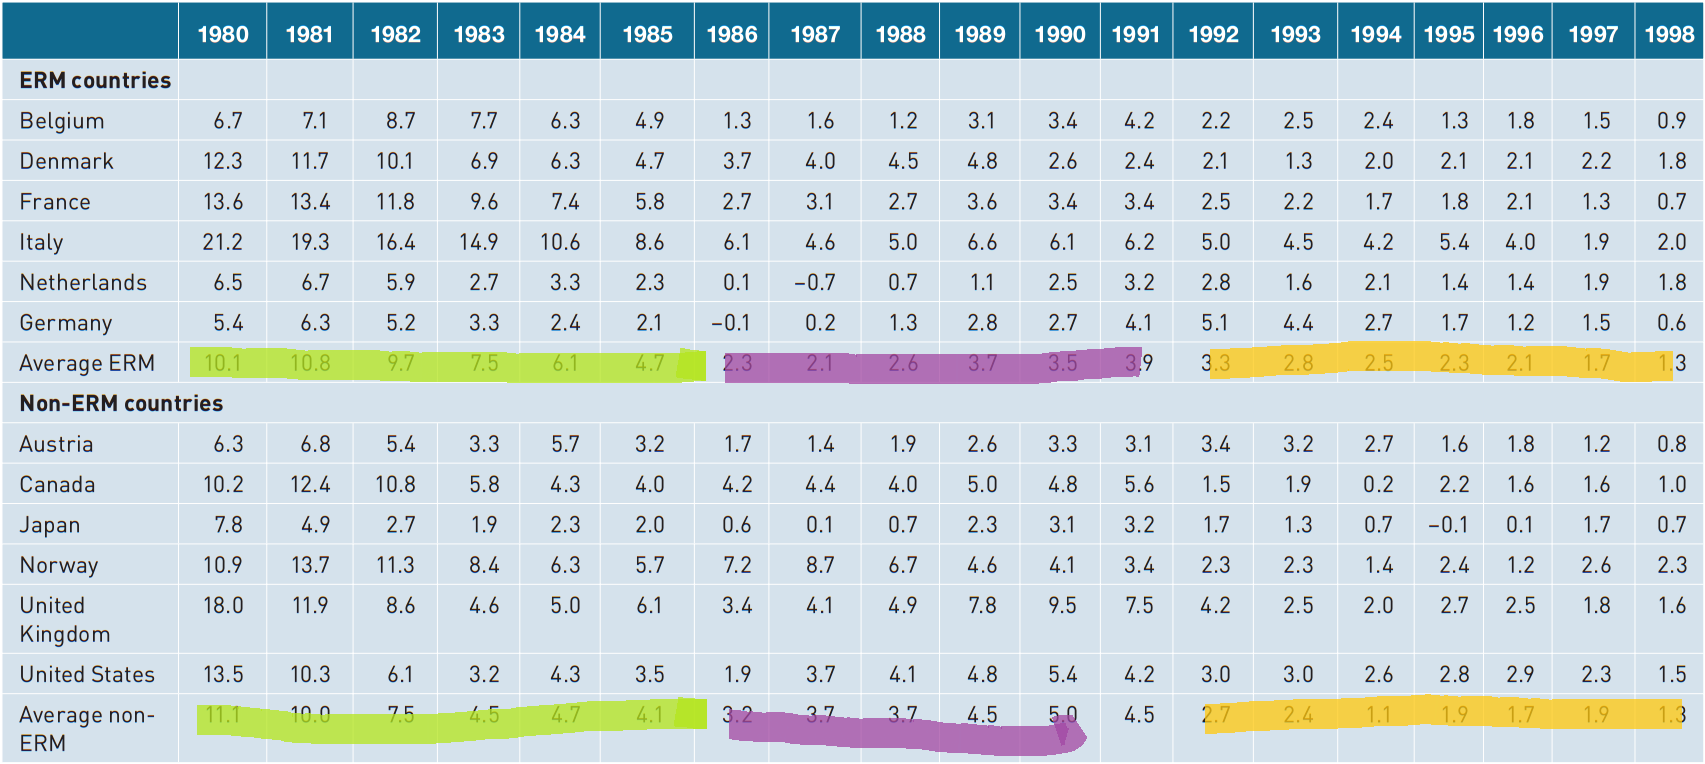
\includegraphics[scale=0.42]{fig/euro/inflation}
\end{frame}

\begin{frame}{The Econommic Performance of ERM and non-ERM Countries}
		\centering
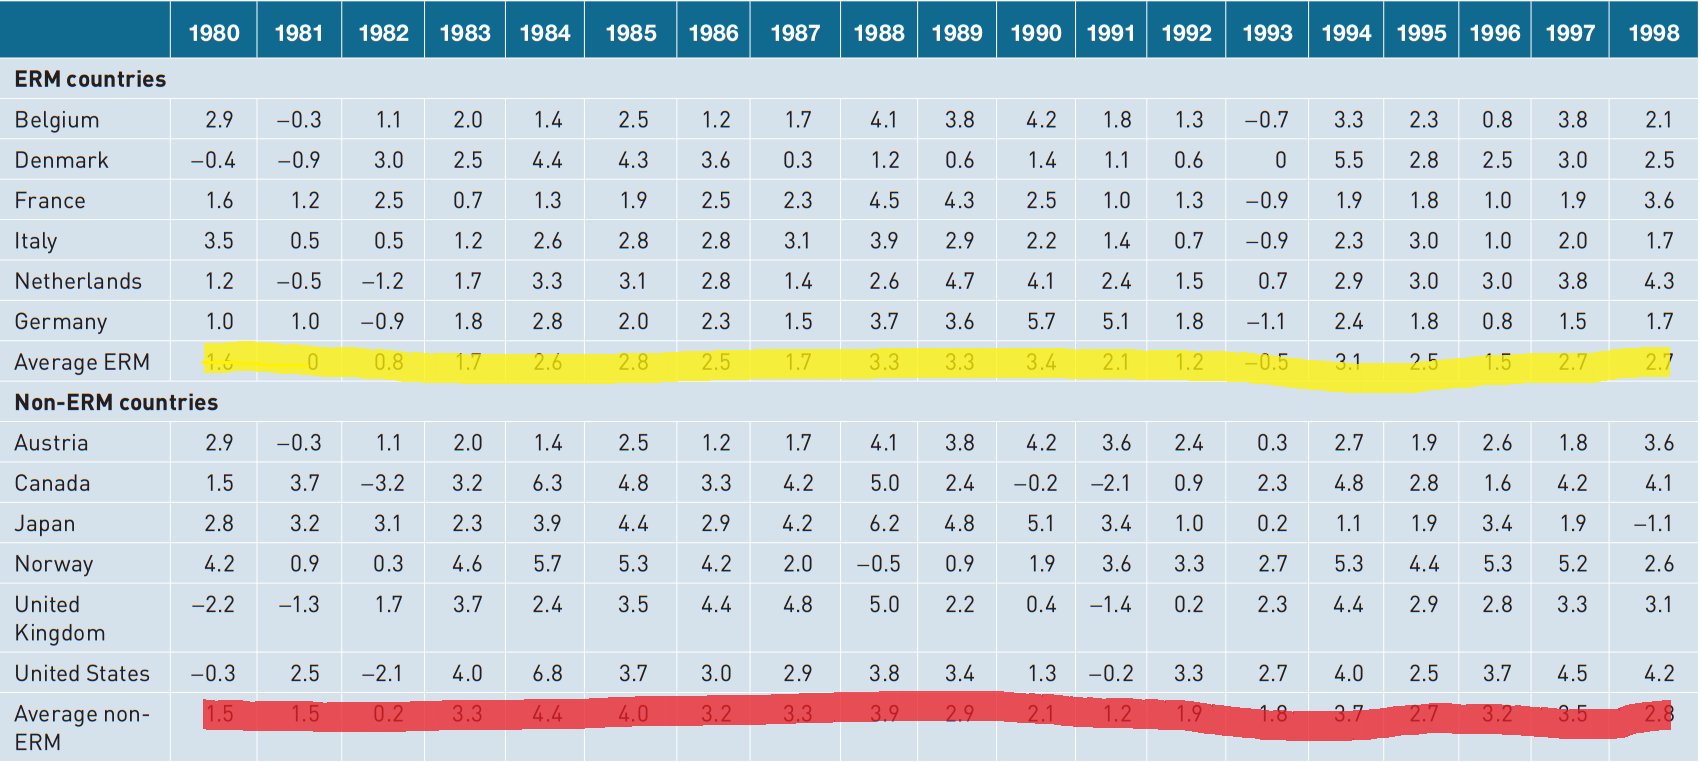
\includegraphics[scale=0.42]{fig/euro/growth}
\end{frame}

\section{From EMS to EMU}
\begin{frame}{What is EMU经济与货币联盟}

	\begin{itemize}
		\item two main components to EMU
		\begin{enumerate}
			\item an exchange rate union 
			\item complete capital market integration
		\end{enumerate}
	\item the difference between Monetary Unit and Fixed Exchange rate regime
			\begin{enumerate}
		\item permanent commitment to fixed exchange rate 
		\item well-developed		institutional framework
		\item capital flow freely
	\end{enumerate}
	\end{itemize}
\end{frame}

\begin{frame}{The Road to EMU in Europe}
	\begin{columns}
		\begin{column}{0.5\textwidth}
			\begin{itemize}
				\item 1957,The Treaty of Rome
				\item 1969,Hague Summit
				\item 1972, The Werner Report
				\item 1989, the Delors Report
			\end{itemize}
		\end{column}
			\begin{column}{0.5\textwidth}
		\begin{itemize}
			\item Stage 1: the convergence phase(1990.7.1-1993.12.31)
			\item Stage 2: the transition phase(1994.1.1-)
			\item Stage 3: the fixing and euro phase(1997.1.1-1999.1.1)

		\end{itemize}
	\end{column}
	\end{columns}
\end{frame}
\begin{frame}{The Maastricht Treaty马斯特里赫特条约}

	\begin{itemize}
		\item As a follow-up to the Delors Report, the Maastricht Treaty was signed in the Dutch
		town of Maastricht in December 1991
		\item The qualification to join EMU
		\begin{enumerate}
			\item Average consumer price inflation in the country should not be more than 1.5\% 
			above that of the three countries with the lowest inflation rates;
			\item A country should not have an excessive budget deficit, with the reference rate
			being that it should not exceed 3\% of GDP;
			\item The outstanding public-sector debt (national debt) of the country should not
			exceed 60\% of GDP;
			\item  Average nominal long-term interest rates in the year of examination should not be
			more than 2\% above that of the three countries with the lowest inflation rates
		\end{enumerate}
	\item two big letout clauses
	\item Special cases for  United Kingdom, Denmark and Sweden.
	\end{itemize}

\end{frame}

\begin{frame}{Evaluation of the Maastricht Criteria}

	\begin{itemize}
		\item The Maastricht criteria were primarily motivated by a German desire to ensure that
		the qualifying members for EMU had a strong fiscal and monetary background.
		\item Criticsim 1: arbitrary both in relation
		to the targets set and the targets chosen
		\item Criticsim 2: the national debt criterion was not really
		appropriate since it looked only on the liability side, ignoring state-owned assets.
		\item Criticsim 3: 与被排除在EMU外相比,高负债国将更容易满足,成为EMU有成员所要求的马斯特里赫特条件。而他们的加入会损害EMU的整体利益
		\item Criticsim 4: the convergence criteria are not really necessary becuase of so-called
		‘no-bail-out’ clause(不救助条款)
		\item Criticsim 5:  there were plenty of ‘before’ conditions but no ‘after’ conditions\\
		如何杜绝加入之后在犯错问题?
	\end{itemize}
\end{frame}

\begin{frame}{The Stability and Growth Pact稳定与增长公约}
	\begin{itemize}
		\item At a summit held in Dublin in December 1996, the Germans secured the SGP.
		\item The purpose is to ensure that fiscal prudence remained in place following the start of EMU
		\item The pact subjects countries running ‘excessive’ fiscal deficits (defined as a deficit above
		3\% of GDP) to fines unless they take action to get their deficits down
		\item There are exceptions: if the member state has suffered a sharp economic downturn, defined as an annual fall of real GDP of 2\%
	\end{itemize}
\end{frame}

\begin{frame}{The Changeover to the Single Currency}
\begin{itemize}
	\item Stage1 (scheduled for May 1998) :  the selection of the countries
	that met the Maastricht criteria and were therefore eligible to join EMU(11 counties are selected)
	\item Stage2 (1 January 1999): the permanent fixing of the bilateral
	rates between the member currencies and announcement of their conversion
	rates to the euro.
	\item State3(starting on 1 January 2002): introduction of euro banknotes
	and coins
\end{itemize}
\end{frame}

\begin{frame}{The Performance of the EURO in the Forgein Exchange Market}
		\centering
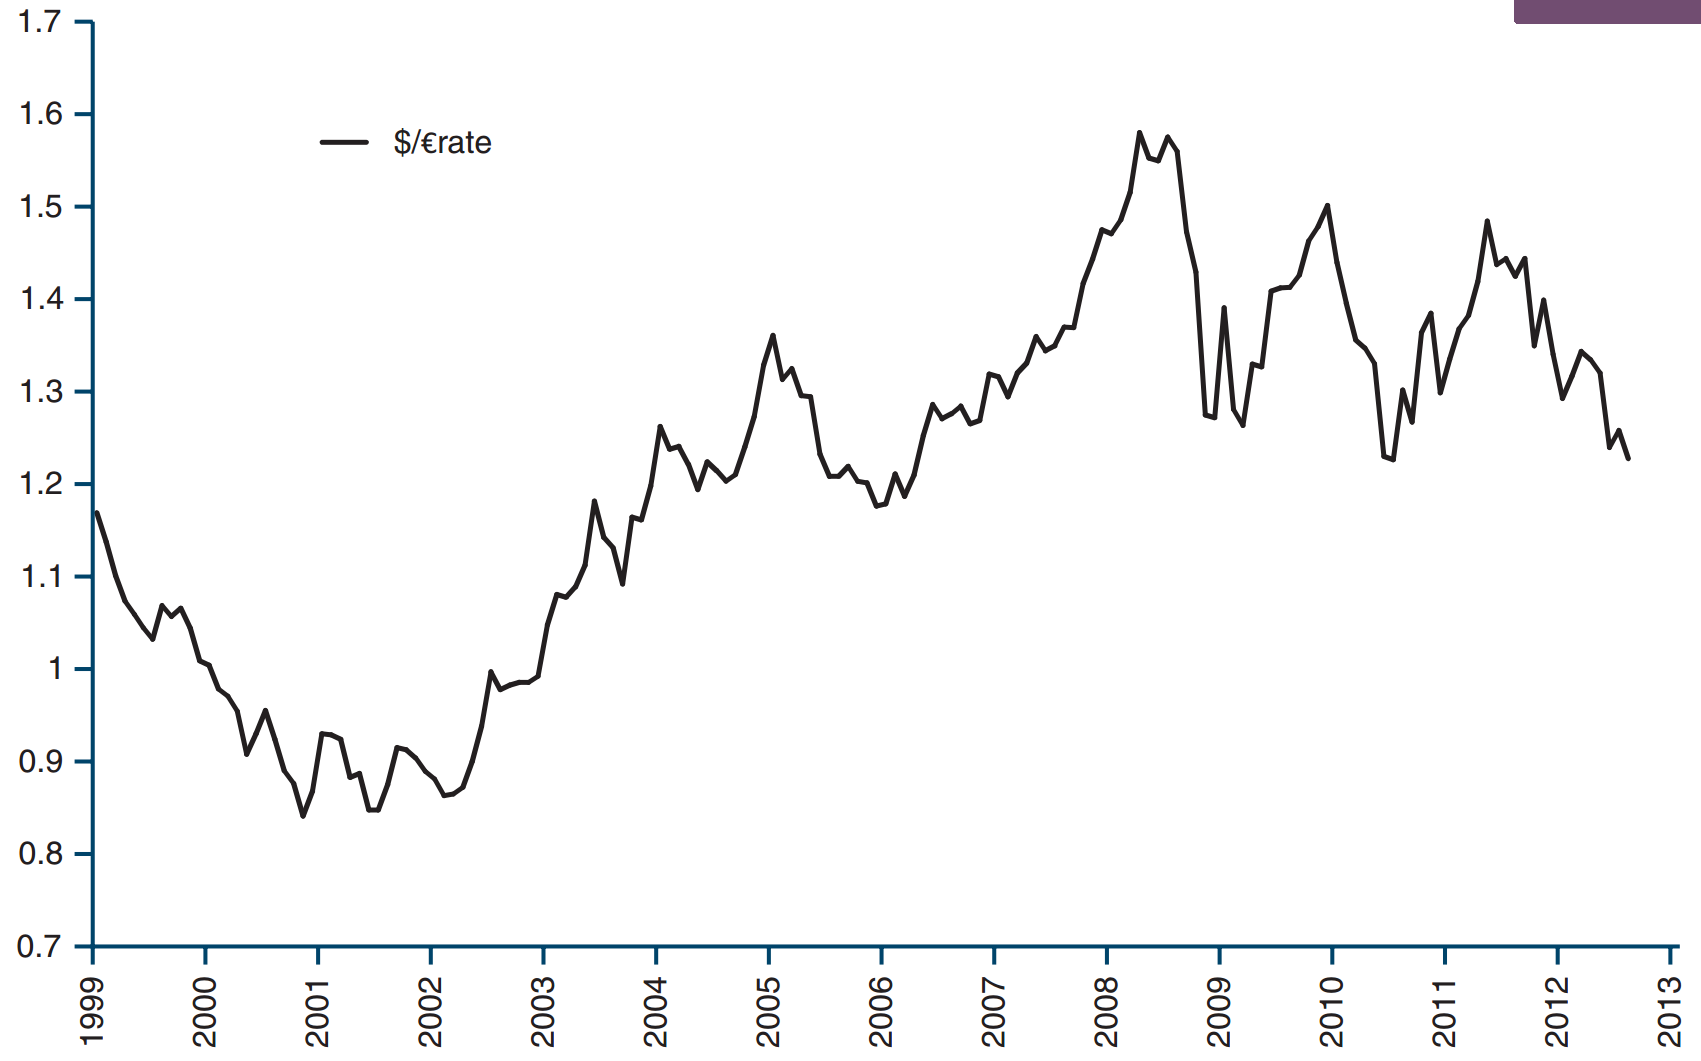
\includegraphics[scale=0.3]{fig/euro/euro}
\end{frame}

\section{the Economics of Euro--- Theory of Optimum Currency Area }
Question:是否应该加入一个最优货币区?做这个决策应该考虑哪些问题?
\begin{itemize}
	\item 主要标准
	\begin{itemize}
		\item Market Integration and Efficiency Benefits 
		\item Economic Symmetry and Stability Costs
	\end{itemize}
	\item 其他标准 
		\begin{itemize}
		\item Labor Market Integration 劳动力市场一体化
		\item Fiscal Transfers 财政转移支付(财政联邦主义)
		\item Monetary Policy and Nominal Anchoring货币政策和名义锚 
		\item Political Objectives 政治目标
	\end{itemize}
\end{itemize}

\begin{frame}{Graphical Illustration: Stylized OCA Criteria}
\centering
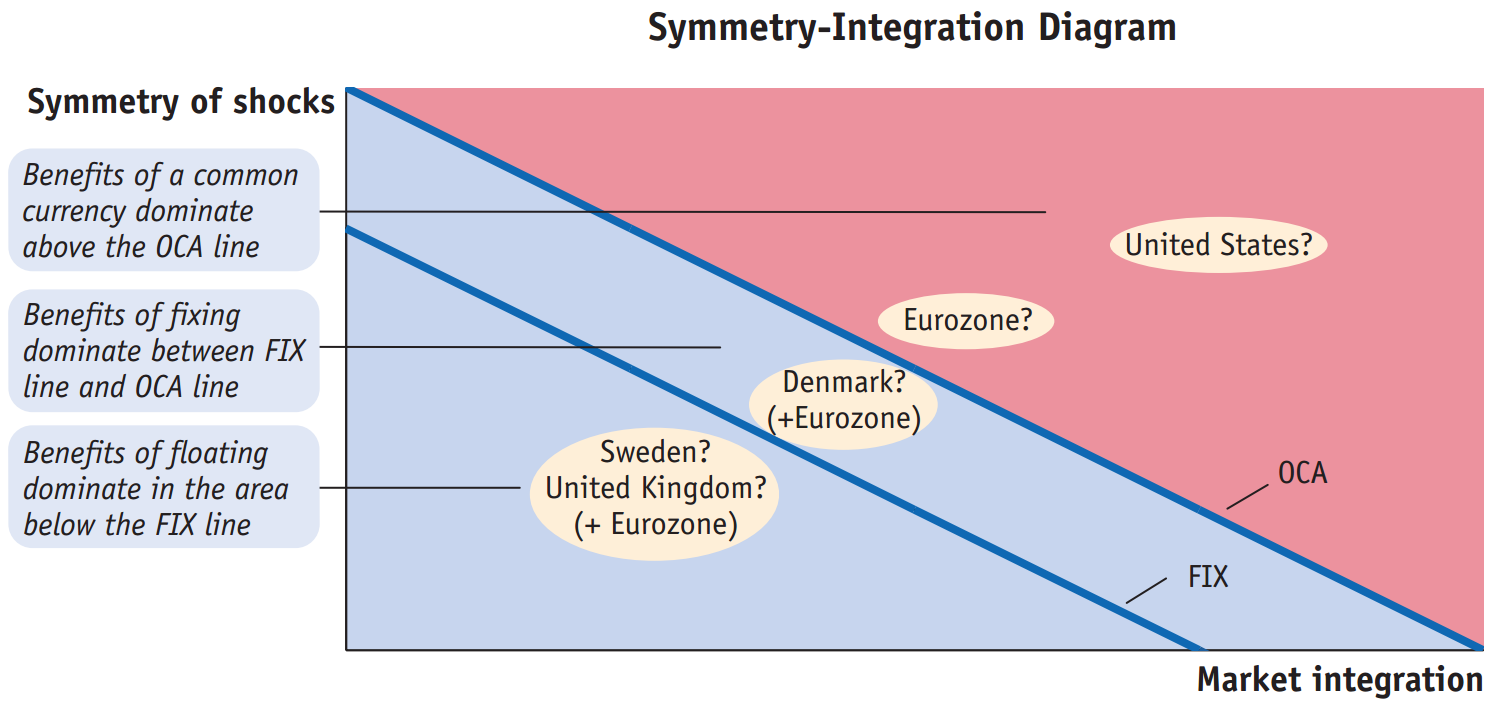
\includegraphics[scale=0.45]{fig/euro/oca2}
\end{frame}

\begin{frame}{OCA Criteria for Europe and the United States比较研究}
		\centering
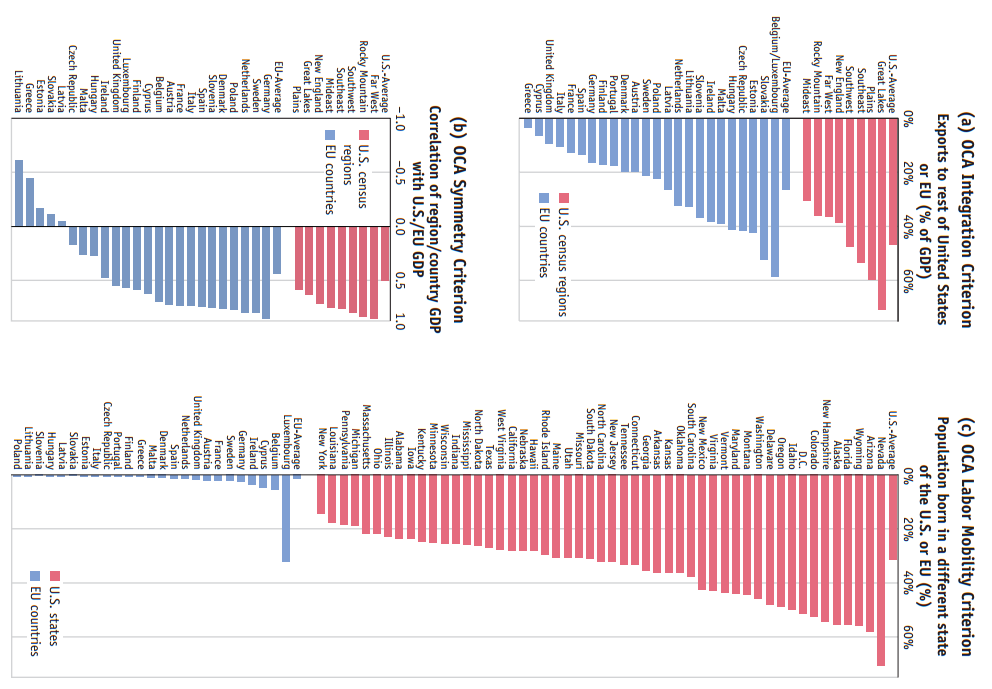
\includegraphics[scale=0.45]{fig/euro/oca}
\end{frame}

\section{the Crisis of EU}

\begin{frame}{the Eurosystem}
	\begin{itemize}
		\item When the ERM I ceased to exist on 1 January 1999, ERM II(欧元预科班) came into being principally
		\item ERM II has four key features
		\begin{enumerate}
			\item  it is based on central rates
			fixed for participating currencies vis-à-vis the euro; no parity grid; the \structure{normal band of fluctuation being ±15\%}
			\item  there exist \structure{obligatory interventions}
			once margins are met; 
			\item the ECB and all participating ‘pre-in’ central banks have	the right to initiate procedures to \structure{review the central rates}
			\item access is provided to \structure{short-term financing facilities} with the ECB having the right to suspend intervention and financing operations.
		\end{enumerate}
	\end{itemize}
\end{frame}

\begin{frame}{an Overview of the EuroSystem}
		\centering
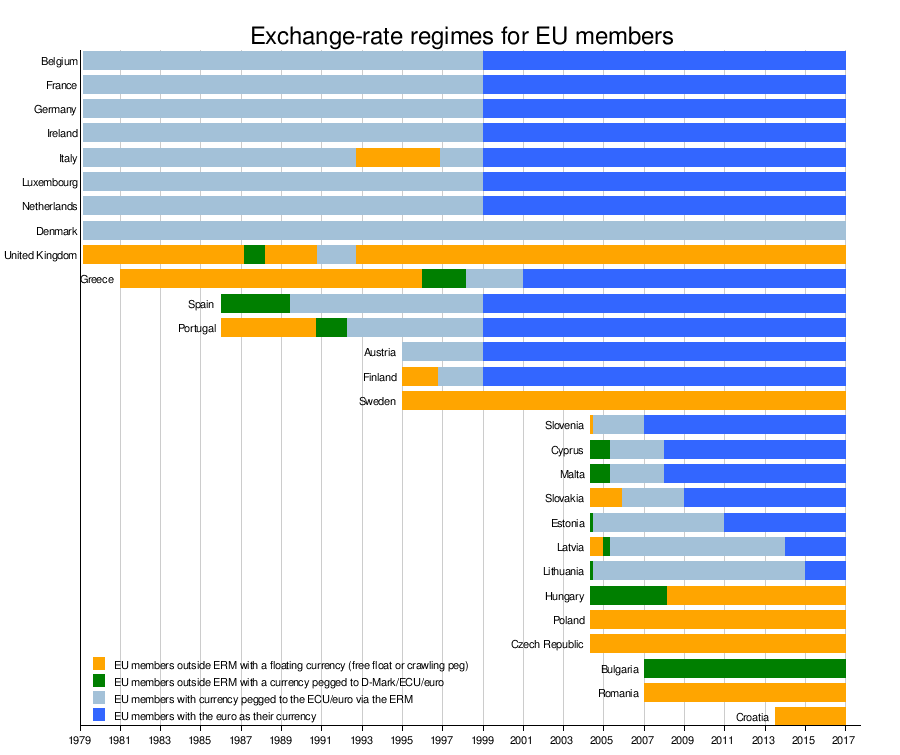
\includegraphics[scale=0.35]{fig/euro/eumember}
\end{frame}

\begin{frame}{PIIGS and the Eurozone Crisis}
	\begin{itemize}
		\item To maintain
		their competitiveness vis-à-vis Germany countries like Portugal, Ireland, Italy, Greece
		and Spain (PIIGS) would need to keep their inflation rates in line with Germany
		\item That is not the case
		\item This loss of competitiveness over time which made them vulnerable
		\item While UIP implies that very short-term interest rates will be equal in a monetary union
		\item the member countries cannot unilaterally	print money to redeem their debt. 
		\item As such, investors have to factor in the possibility that a country that has issued bonds may default on its obligations.
		\item  once the credit crunch got under way, PIIGS debt are given up and attacked
		\item Greece---Ireland---Poutugal---Itlay---Spain
	\end{itemize}
\end{frame}

\begin{frame}{Credit Crisis}
\begin{columns}[onlytextwidth]
\begin{column}{0.5\textwidth}
			\centering
	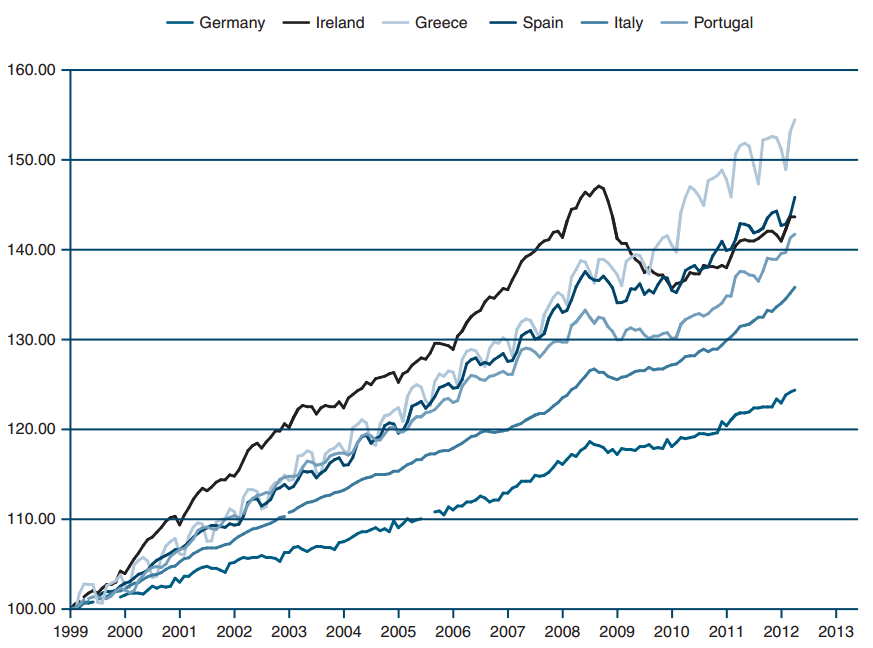
\includegraphics[scale=0.35]{fig/euro/inflation2}
\end{column}
\begin{column}{0.5\textwidth}
	\centering
	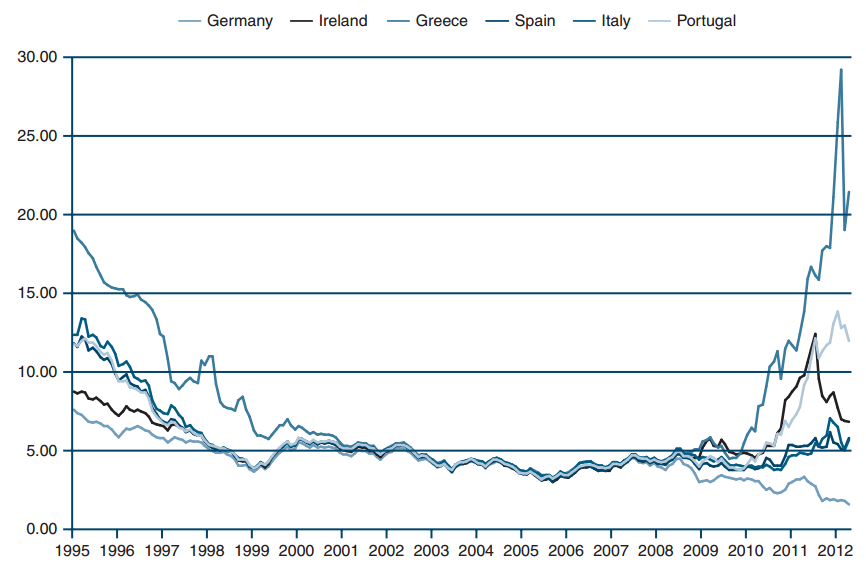
\includegraphics[scale=0.33]{fig/euro/bond}
\end{column}
\end{columns}

\end{frame}

\begin{frame}{The bailous of PIIGS}
		\begin{itemize}
			\item 不是有“不救助条款”(no bailout clause)吗?为什么要救?
			\item the other measures to save them
			\begin{itemize}
				\item 资产担保债权购买计划 Covered Bond Purchase Programme(CBPP)
				\item 证券市场项目 Securities Market	Programme (SMP)
				\item 长期再融资操作 Long Term Refinancing Operation (LTRO)
				\item 2012年,签订《财政稳定条约》(( Fiscal Stability
				Treaty)		
				\item 	欧洲稳定机制 European Stability Mechanism
				\item 直接货币交易计划 Outright MonetaryThe European Monetary System Transactions (OMTs)
							
		\end{itemize}
		\end{itemize}
\end{frame}

\begin{frame}{Proposals to resolve the european debt crisis}
	\begin{itemize}
	\item 结构化改革 Structural reform
	\item 债务减免/重组 Debt forgiveness/restructuring
	\item 发行共同欧元债券 The issuance of common E-bonds (eurobonds)
	\item 允许欧洲央行印欧元来担保债务偿还 Allow the ECB to print euros to guarantee debt repayment
	\item 银行联盟 A Banking Union
\end{itemize}
\begin{block}{Openning Question}
	What's your opinoion on the outlook of Euro?
\end{block}
\end{frame}

\end{document}


